\documentclass[pdf]{beamer}
\usepackage{listings}
\usepackage{adjustbox}
\usetheme{Luebeck} %default, AnnArbor, Antibes, Bergen, Berkeley, Berlin, Boadilla, CambridgeUS, Copenhagen, Darmstadt, Dresden, EastLansing, Frankfurt, Goettingen, Hannover, Ilmenau, JuanLesPins, Luebeck, Madrid, Malmoe, Marburg, Montpellier, PaloAlto, Pittsburgh, Rochester, Singapore, Szeged, Warsaw

\usecolortheme{beaver} %default, albatross, beaver, beetle, crane, dolphin, dove, fly, lily, orchid, rose, seagull, seahorse, whale, wolverine
%\useinnertheme{circle} %circles, rectangles, rounded, inmargin 
%\useoutertheme{tree} %infolines, smoothbars, sidebar, split, tree 

\definecolor{coqatoo-pink}      {RGB}{255, 107, 104}
\definecolor{coqatoo-gray}      {RGB}{64, 64, 64}
\definecolor{coqatoo-yellow}    {RGB}{239, 223, 0}

\setbeamercolor{palette primary}   {bg=coqatoo-pink,fg=white}
%\setbeamercolor{palette secondary} {bg=white,fg=black}
%\setbeamercolor{palette tertiary}  {bg=blue,fg=red}
%\setbeamercolor{palette quaternary}{bg=white,fg=black}
\setbeamercolor{structure}{fg=coqatoo-gray}
\setbeamercolor{titlelike}         {bg=coqatoo-pink,fg=white}
\setbeamercolor{frametitle}        {bg=coqatoo-pink,fg=white}
\setbeamercolor{normal text}       {bg=white,fg=coqatoo-gray}
\newcommand{\coqatoo}{Coqatoo}


\definecolor{grey}{rgb}{0.8,0.8,0.8}
\definecolor{code-background}{RGB}{255, 248, 220}
\definecolor{code-comment}{RGB}{196, 42, 42}
\definecolor{code-linenumber}{rgb}{0.5,0.5,0.5}
\definecolor{code-keyword}{RGB}{148, 0, 211}
\lstset{
   backgroundcolor=\color{code-background},   	% choose the background color; you must add \usepackage{color} or \usepackage{xcolor}
   basicstyle=\tt\small,       			% the size of the fonts that are used for the code
   breakatwhitespace=false,         			% sets if automatic breaks should only happen at whitespace
   breaklines=true,                 			% sets automatic line breaking
   captionpos=none,                    			% sets the caption-position to bottom
   commentstyle=\color{code-comment},   		% comment style
   deletekeywords={...},            			% if you want to delete keywords from the given language
   escapeinside={\%*}{*)},          			% if you want to add LaTeX within your code
   extendedchars=true,              			% lets you use non-ASCII characters; for 8-bits encodings only, does not work with UTF-8
   frame=tb,
   framerule=0pt,
   framextopmargin=0pt,
   framexbottommargin=0pt,
   keepspaces=true,                 			% keeps spaces in text, useful for keeping indentation of code (possibly needs columns=flexible)
   keywordstyle=\color{code-keyword},       						% keyword style
   language=ML,                 				% the language of the code
   morekeywords={Lemma, Proof, Qed},            % if you want to add more keywords to the set
   numbers=none,                    			% where to put the line-numbers; possible values are (none, left, right)
   numbersep=5pt,	                   			% how far the line-numbers are from the code
   numberstyle=\tiny\color{code-linenumber}, 	% the style that is used for the line-numbers
   rulecolor=\color{black}, 	        		% if not set, the frame-color may be changed on line-breaks within not-black text (e.g. comments (green here))
   showspaces=false,            	    		% show spaces everywhere adding particular underscores; it overrides 'showstringspaces'
   showstringspaces=false,          			% underline spaces within strings only
   showtabs=false,                  			% show tabs within strings adding particular underscores
   stepnumber=1,                    			% the step between two line-numbers. If it's 1, each line will be numbered
   stringstyle=\color{black},            		% string literal style
   tabsize=2,                       			% sets default tabsize to 2 spaces
   gobble=0,									% number of characters to remove at the beginning of each line
   mathescape=true,								% to render math symbols in the listing (between $)
   title=\lstname,                   			% show the filename of files included with \lstinputlisting; also try caption instead of title
   belowcaptionskip = 0cm
}

\title[Coqatoo]{
\includegraphics[width=50pt]{images/logo.png}\\Coqatoo}
\subtitle{Generating Natural Language Versions of Coq Proofs}
\author{Andrew Bedford}
\institute{Laval University}
\date{CoqPL 2018}
\expandafter\def\expandafter\insertshorttitle\expandafter{%
\insertshorttitle\hfill%
\insertframenumber\,/\,\inserttotalframenumber}
\begin{document}

\begin{frame}
    \titlepage
\end{frame}

\begin{frame}{Motivation}
Scenarios where having the natural-language version of a Coq proof could be useful:
\begin{enumerate}
    \item Learning
    \item Communicating
    \item Documenting
\end{enumerate}
~\\
You could manually write natural-language version of your proofs, but...
\end{frame}

\begin{frame}[fragile]{Example}{Input}
\begin{adjustbox}{minipage=\linewidth,bgcolor=coqatoo-gray,trim=-3pt 5pt -3pt 5pt}        
\begin{lstlisting}[label=listing:input]
Lemma conj_imp_equiv : forall P Q R:Prop, 
  (P /\ Q -> R) <-> (P -> Q -> R).
Proof.
  intros. split. intros H HP HQ. apply H. apply conj. assumption. assumption. 
  intros H HPQ. inversion HPQ. apply H. assumption. assumption.
Qed.
\end{lstlisting}
\end{adjustbox}
\end{frame}

\begin{frame}[fragile]{Example}{Output (--mode text)}
\begin{adjustbox}{minipage=\linewidth,bgcolor=coqatoo-gray,trim=-3pt 5pt -3pt 5pt}
\begin{lstlisting}[keywordstyle=\color{white}]
Given any P, Q and R : Prop. Let us show that (P /\ Q -> R) <-> (P -> Q -> R) is true.
- Case (P /\ Q -> R) -> P -> Q -> R:
    Suppose that P, Q, P /\ Q -> R are true. Let us show that R is true.
    By our hypothesis P /\ Q -> R, we know that R is true if P /\ Q are true.
    -- Case P:
       True, because it is one of our assumptions.
    -- Case Q:
       True, because it is one of our assumptions.
- Case (P -> Q -> R) -> P /\ Q -> R:
    Suppose that P /\ Q, P -> Q -> R are true. Let us show that R is true.
    By our hypothesis P -> Q -> R, we know that R is true if P, Q are true.
    -- Case P:
       True, because it is one of our assumptions.
    -- Case Q:
       True, because it is one of our assumptions.
\end{lstlisting}
\end{adjustbox}
\end{frame}

\begin{frame}[fragile]{Example}{Output (--mode coq)}
\begin{adjustbox}{minipage=\linewidth,bgcolor=coqatoo-gray,trim=-3pt 5pt -3pt 5pt}
\begin{lstlisting}[label=listing:output]
Lemma conj_imp_equiv : forall P Q R:Prop, (P /\ Q -> R) <-> (P -> Q -> R).
Proof.
  (* Given any P, Q, R : Prop. Let us show that (P /\ Q -> R) <-> (P -> Q -> R) is true. *) intros.
  split.
  - (* Case (P /\ Q -> R) -> P -> Q -> R: *) 
    (* Suppose that P, Q and P /\ Q -> R are true. Let us show that R is true. *) intros H HP HQ.
    (* By our hypothesis P /\ Q -> R, we know that R is true if P /\ Q  is true. *) apply H.
    apply conj.
    -- (* Case P: *)
       (* True, because it is one of our assumptions. *) assumption.
    -- (* Case Q: *)
       (* True, because it is one of our assumptions. *) assumption.
  - (* Case (P -> Q -> R) -> P /\ Q -> R: *)
    (* Suppose that P /\ Q and P -> Q -> R are true. Let us show that R is true. *) intros H HPQ.
    (* By inversion on P /\ Q, we know that P, Q are also true. *) inversion HPQ.
    (* By our hypothesis P -> Q -> R, we know that R is true if P and Q are true. *) apply H.
    -- (* Case P: *)
       (* True, because it is one of our assumptions. *) assumption.
    -- (* Case Q: *)
       (* True, because it is one of our assumptions. *) assumption.
Qed.
\end{lstlisting}
\end{adjustbox}
\end{frame}

\begin{frame}{Example}{Output (--mode latex)}
    \begin{lemma} (conj\_imp\_equiv) $\forall P, Q, R : Prop, (P \land Q \Rightarrow R) \Leftrightarrow (P \Rightarrow Q \Rightarrow R)$
    \end{lemma}
    \begin{proof}\scriptsize
        Given any $P, Q~and~R : Prop$. Let us show that $(P \land Q \Rightarrow R) \Leftrightarrow (P \Rightarrow Q \Rightarrow R)$ is true.\\
\hspace{5mm}- Case $(P \land Q \Rightarrow R) \Rightarrow P \Rightarrow Q \Rightarrow R$:\\
\hspace{5mm}\hspace{5mm}Suppose that $P, Q, P \land Q \Rightarrow R$ are true. Let us show that $R$ is true.\\
\hspace{5mm}\hspace{5mm}By our hypothesis $P \land Q \Rightarrow R$, we know that $R$ is true if $P \land Q$ are true.\\
\hspace{5mm}\hspace{5mm}-- Case $P$:\\
\hspace{5mm}\hspace{5mm}\hspace{5mm}True, because it is one of our assumptions.\\
\hspace{5mm}\hspace{5mm}-- Case $Q$:\\
\hspace{5mm}\hspace{5mm}\hspace{5mm}True, because it is one of our assumptions.\\
\hspace{5mm}- Case $(P \Rightarrow Q \Rightarrow R) \Rightarrow P \land Q \Rightarrow R$:\\
\hspace{5mm}\hspace{5mm}Suppose that $P \land Q, P \Rightarrow Q \Rightarrow R$ are true. Let us show that $R$ is true.\\
\hspace{5mm}\hspace{5mm}By our hypothesis $P \Rightarrow Q \Rightarrow R$, we know that $R$ is true if $P, Q$ are true.\\
\hspace{5mm}\hspace{5mm}-- Case $P$:\\
\hspace{5mm}\hspace{5mm}\hspace{5mm}True, because it is one of our assumptions.\\
\hspace{5mm}\hspace{5mm}-- Case $Q$:\\
\hspace{5mm}\hspace{5mm}\hspace{5mm}True, because it is one of our assumptions.\\
    \end{proof}
\end{frame}

\begin{frame}{Languages}
    \begin{itemize}
        \item Can generate proofs in multiple languages
        \item Easy to add support for additional languages
        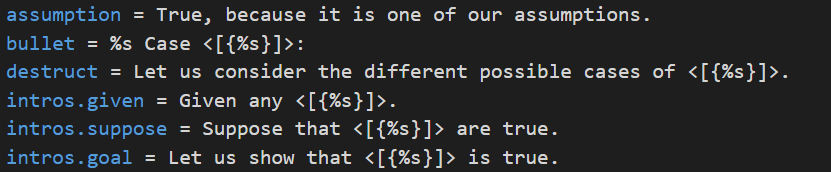
\includegraphics[width=\textwidth]{images/sentences.png}
    \end{itemize}
\end{frame}

\begin{frame}{Overview of Coqatoo}
    Coqatoo's rewriting algorithm can be decomposed in three steps:
    \begin{enumerate}
        \item Information extraction
        \item Proof tree construction
        \item Tactic-based rewriting
    \end{enumerate}
\end{frame}


\begin{frame}[fragile]{Step 1: Information extraction}
\begin{adjustbox}{minipage=\linewidth,bgcolor=coqatoo-gray,trim=-3pt 5pt -3pt 5pt}
\begin{lstlisting}[label=listing:before-intros]
1 subgoal

============================
forall P Q R : Prop, (P /\ Q -> R) <-> (P -> Q -> R)
\end{lstlisting}
\end{adjustbox}
\vspace{0.25cm}~\\
intros.\\
\vspace{0cm}~\\
\begin{adjustbox}{minipage=\linewidth,bgcolor=coqatoo-gray,trim=-3pt 5pt -3pt 5pt}
\begin{lstlisting}[label=listing:after-intros]
1 subgoal

P, Q, R : Prop
============================
(P /\ Q -> R) <-> (P -> Q -> R)
\end{lstlisting}
\end{adjustbox}
\end{frame}

\begin{frame}{Step 2: Proof tree construction}
    \vspace{-13pt}\center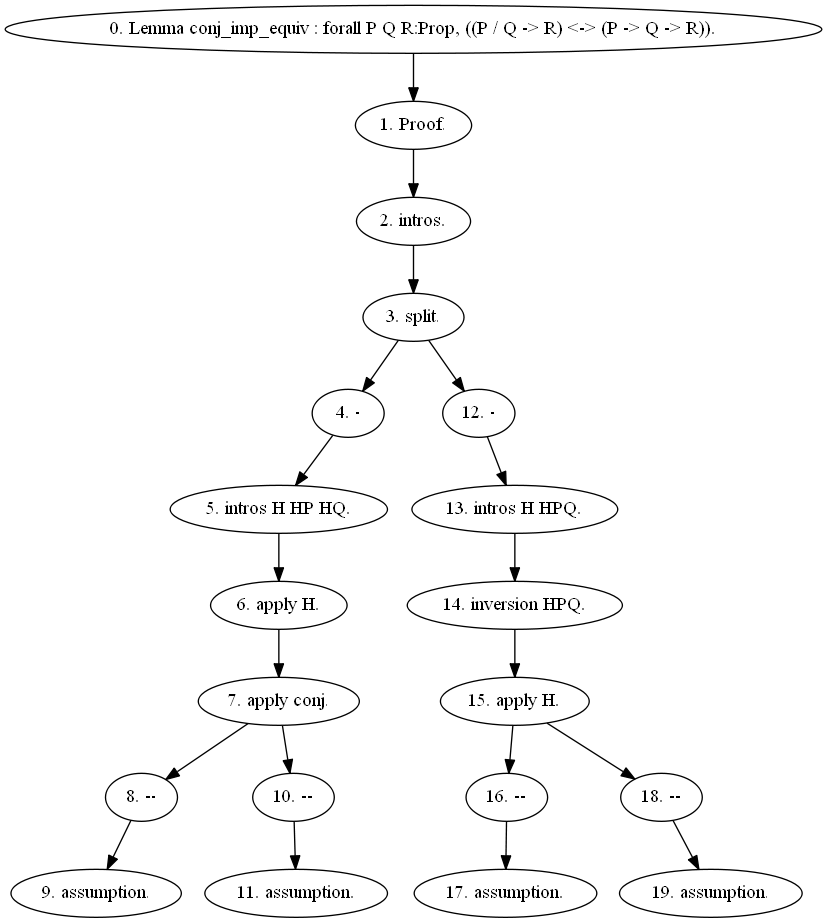
\includegraphics[height=0.85\textheight]{images/proof-tree.png}
\end{frame}

\begin{frame}{Step 3: Tactic-based rewriting}
Each supported tactic has its own set of rules. Take {\tt intros} for example:
\begin{itemize}
    \item If variables are introduced, then {\tt Given any...}
    \item If hypotheses are introduced, then {\tt Suppose...}
    \item {\tt Let us prove...}
\end{itemize}
\end{frame}

\begin{frame}[fragile]{Related Work}{CtCoq and PCoq}


\begin{adjustbox}{minipage=\linewidth,bgcolor=coqatoo-gray,trim=-3pt 5pt -3pt 5pt}            
\begin{lstlisting}
conj_imp_equiv = 
fun P Q R : Prop =>
conj (fun (H : P /\ Q -> R) (HP : P) (HQ : Q) => H (conj HP HQ))
    (fun (H : P -> Q -> R) (HPQ : P /\ Q) =>
    let H0 :=
        match HPQ with
        | conj H0 H1 => (fun (H2 : P) (H3 : Q) => H H2 H3) H0 H1
        end
        :
        R in
    H0)
        : forall P Q R : Prop, (P /\ Q -> R) <-> (P -> Q -> R)
\end{lstlisting}
\end{adjustbox}
\end{frame}


\begin{frame}{Comparison}{Advantages / Disadvantages}
    Disadvantages
    \begin{itemize}
        \item{It only works on proofs whose tactics are supported, while the approach of Coscoy et al. worked on any proof.}
        \item{Won't work well if there is a lot of automation}
    \end{itemize}

    Advantages
    \begin{itemize}
        \item{It enables us to more easily control the size and verbosity of the generated proof (one or two sentences per tactic by default).}
        \item{It maintains the order and structure of the user's original proof script; this is not necessarily the case in Coscoy et al. }
      \end{itemize}
\end{frame}

\begin{frame}{Future work}
    \begin{itemize}
        \item Increase the number of supported tactics
        \begin{itemize}
            \item Currently supports only a handful
            \item Goal: Software Foundations
        \end{itemize}
        \item Add partial support for automation
        \item Add support for other languages 
        \item Integration with existing development environments
    \end{itemize}
\end{frame}

\begin{frame}{}{}
    \center {\Huge Thank you!}\\~\\
    github.com/andrew-bedford/coqatoo
\end{frame}

\end{document}